%% V1.0
%% by Gabriel Garcia, gabrcg@gmail.com
%% This is a template for Udacity projects using IEEEtran.cls

%% Be Udacious!

\documentclass[10pt,journal,compsoc]{IEEEtran}

\usepackage[pdftex]{graphicx}    
\usepackage{cite}
\usepackage{hyperref}
% \documentclass{article}
\usepackage{listings}
\usepackage{xcolor} % for setting colors

% set the default code style
\lstset{
    frame=tb, % draw a frame at the top and bottom of the code block
    tabsize=4, % tab space width
    showstringspaces=false, % don't mark spaces in strings
    % numbers=left, % display line numbers on the left
    commentstyle=\color{green}, % comment color
    keywordstyle=\color{blue}, % keyword color
    stringstyle=\color{red} % string color
}
\hyphenation{op-tical net-works semi-conduc-tor}


\begin{document}

\title{Deep RL Arm Manipulation}

\author{Ghee Chong Foo}

\markboth{Deep RL Arm Manipulation, Robotics Nanodegree Program, Udacity}%
{}
\IEEEtitleabstractindextext{%

\begin{abstract}
In this project, a robotic arm was trained through reinforcement learning, using Deep Q-Learning networking, with the objective of different part of the arm touching the object with desired accuracy.

\end{abstract}

% Note that keywords are not normally used for peerreview papers.
\begin{IEEEkeywords}
Robotics, DeepRL.
\end{IEEEkeywords}}


\maketitle
\IEEEdisplaynontitleabstractindextext
\IEEEpeerreviewmaketitle
\section{Introduction}
\label{sec:introduction}

\IEEEPARstart
{T}his project explores the feasibility of manipulating a robotic arm using Deep RL (reinforcement learning) in a gazebo environment and arm plugin (ArmPlugin.cpp) which assigns positive or negative rewards when the arm touches the object with different part of the arm, or misses it by touching the ground. 

Figure \ref{fig:Arm_init_pos} shows the setup for the project.  The gazebo plugin, namely ArmPlugin.cpp will subscribe to camera and contact/collision node which is then pass on to the DQN agent as input.  Code snipppet as below:

\begin{lstlisting}[language=C++]
cameraSub =  cameraNode->Subscribe( 
"/gazebo/arm_world/camera/link/camera/image",
&gazebo::ArmPlugin::onCameraMsg, this);
            
collisionSub = collisionNode->Subscribe( 
"/gazebo/arm_world/tube/tube_link/my_contact",
&gazebo::ArmPlugin::onCollisionMsg, this);
\end{lstlisting}


%{T}{he} introduction should provide some material regarding the history of the problem, why it is important and what is intended to be achieved. If there exists any previous attempts to solve this problem, this is a great place to note these while conveying the differences in your approach (if any). The intent is to provide enough information for the reader to understand why this problem is interesting and setting up the conversation for the solution you have provided
%Use this space to introduce your localization task and how you wish to accomplish it; save the details about the robot construction for later (simulation is a good point for this information). 
%If you have any papers / sites / repositories you have referenced for your robot, please make sure to cite them.

%example for inserting image
\begin{figure}[thpb]
      \centering
      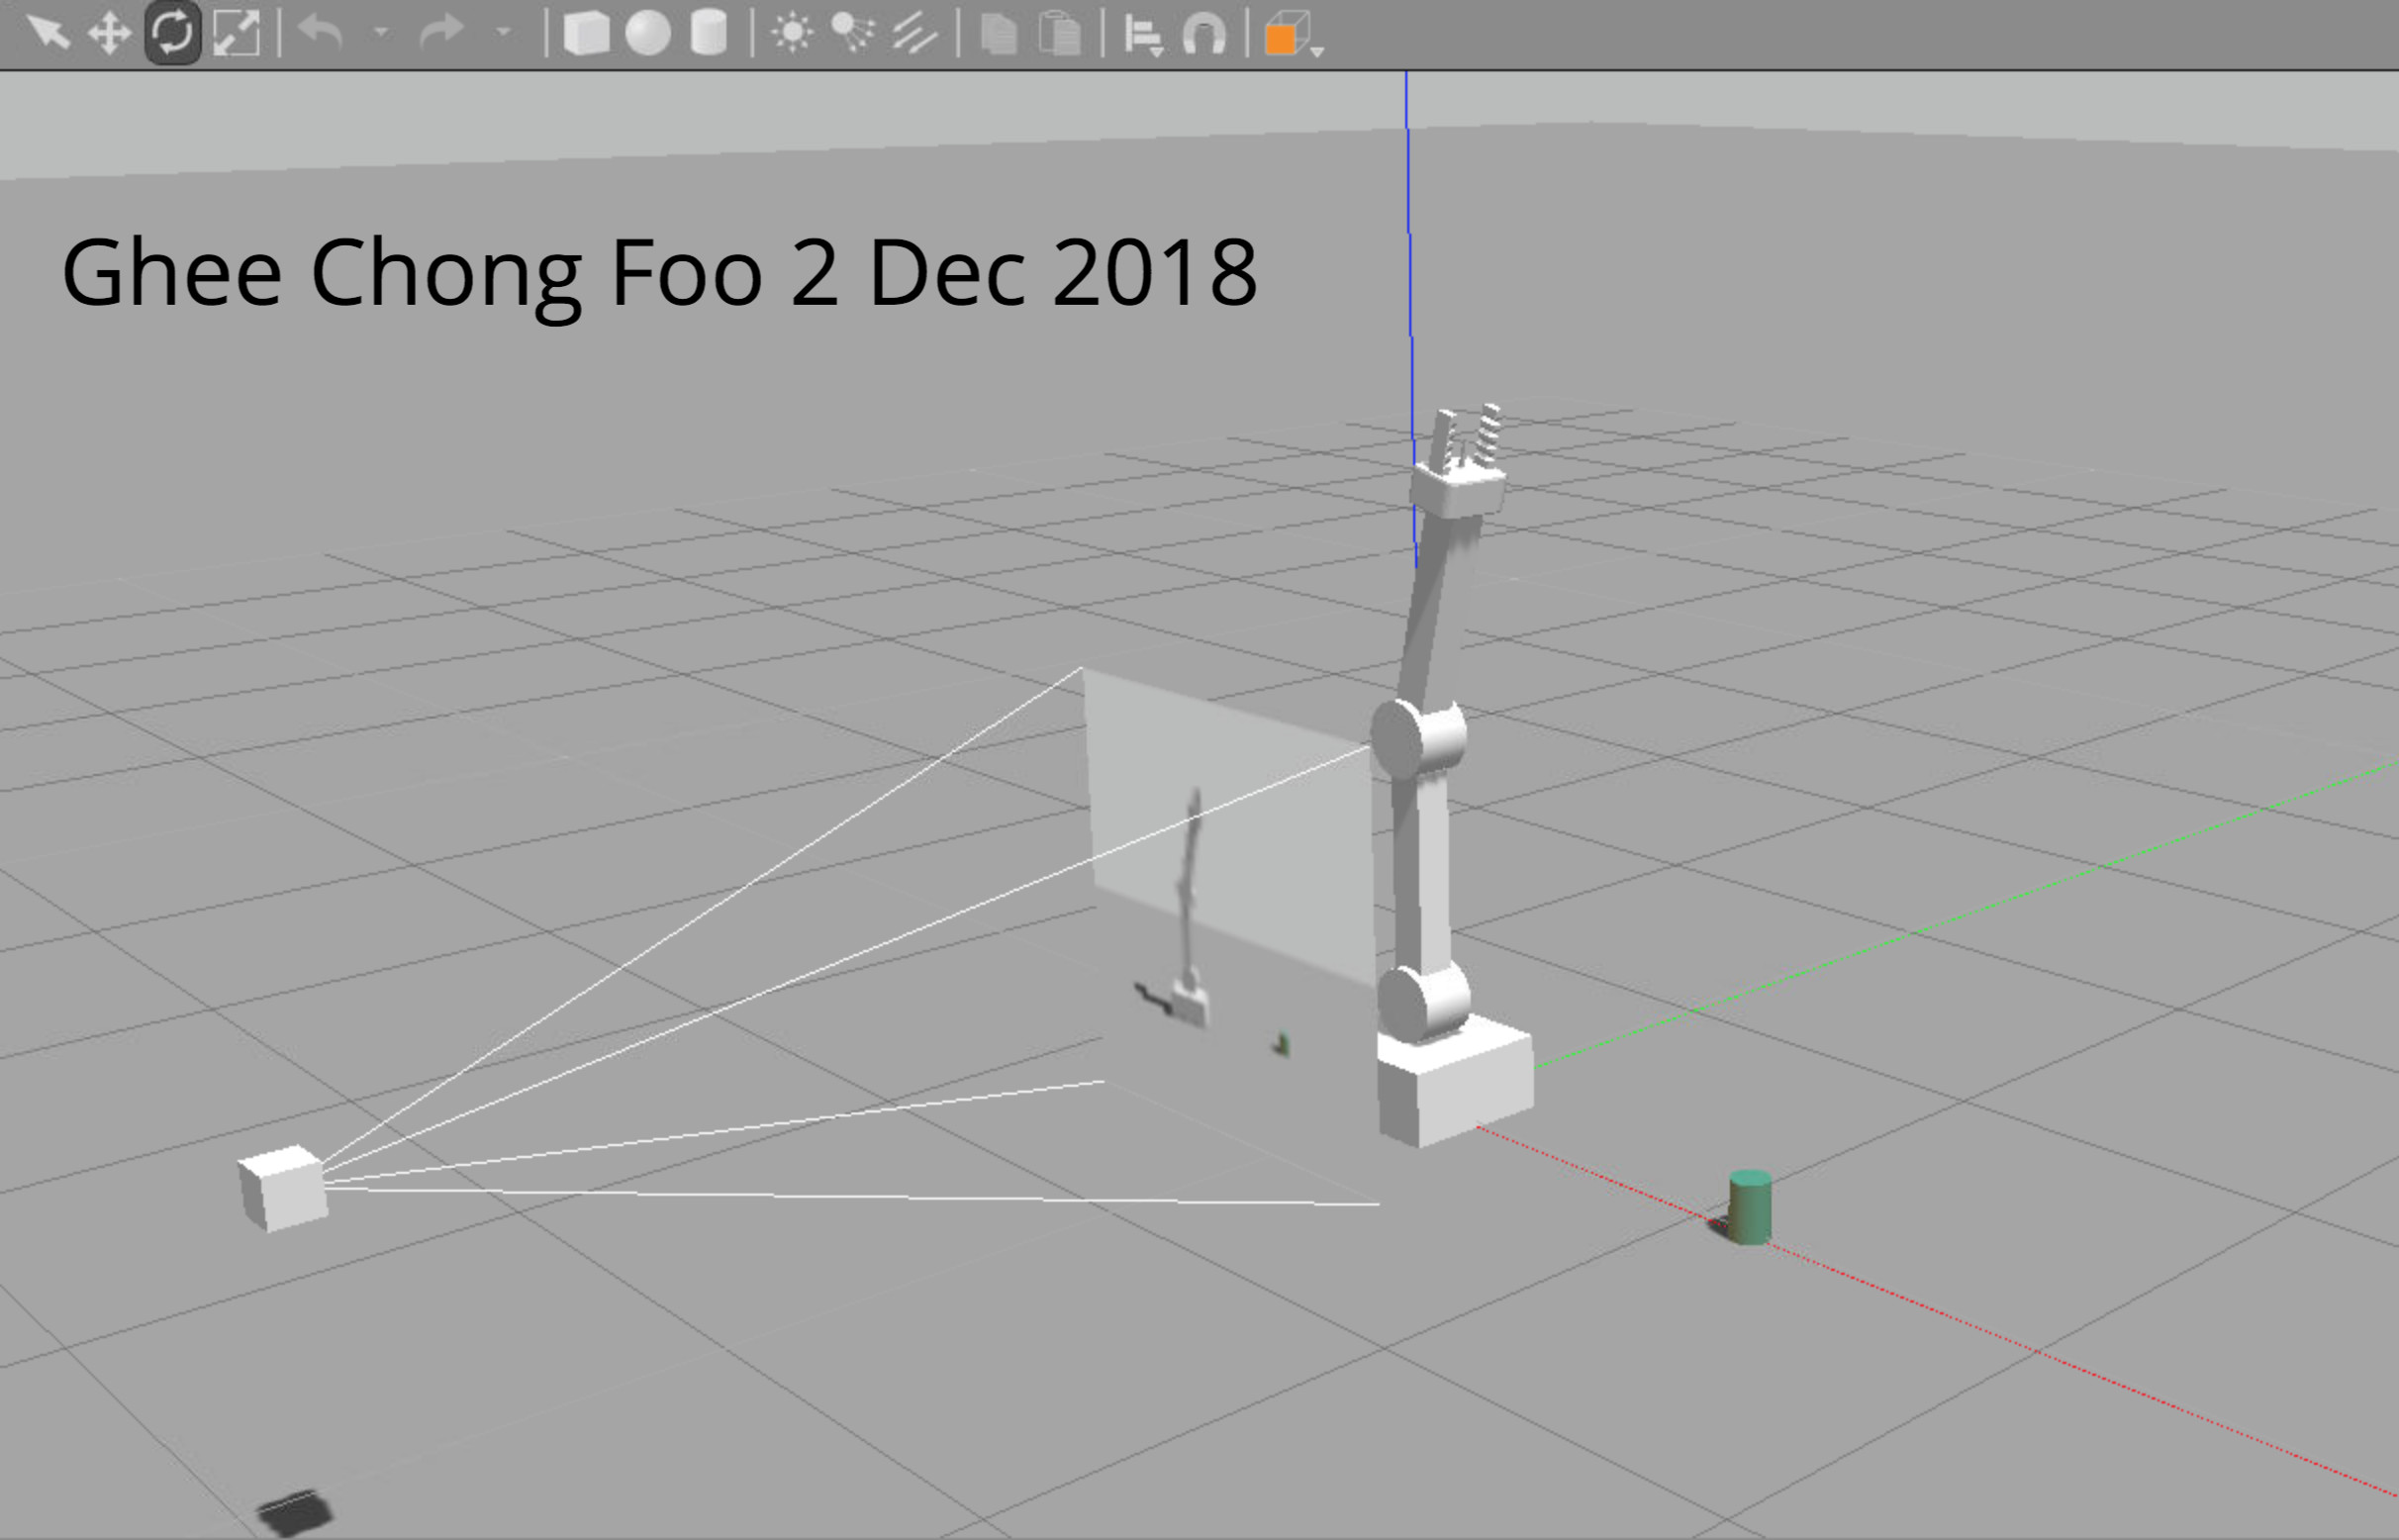
\includegraphics[width=\linewidth]{Arm_init_pos.png}
      \caption{Robotic Arm Initial Position}
      \label{fig:Arm_init_pos}
\end{figure}

%\subsection{Subsection Heading Here}
%Subsection text here.

%\subsubsection{Subsubsection Heading Here}
%Subsubsection text here.

%example for building table
%\begin{table}[h]
%\caption{Table}
%\label{table_example}
%\begin{center}
%\begin{tabular}{|c||c|}
%\hline
%One & Two\\
%\hline
%Three & Four\\
%\hline
%\end{tabular}
%\end{center}
%\end{table}



\section{Reward Functions}

Three types of rewards are defined:
\begin{enumerate}
    \item \textbf{Win}: Reward is issued when the robotic arm achieve the objective and ending the episode with a success.
    \item \textbf{Loss}: Penalty issued when robotic arm misses the objectives or hitting undesirable location.  This ends the episode with a failure
    \item \textbf{Interim}: Interim reward is issued while robot is moving and episode still running. This will guide the agent to move the robot in the desired direction and will be positive or negative depending on position of the arm.
\end{enumerate}


\subsection{Win Reward}
Positive reward is issued when robot arm touches the object.  In challenge 1, reward is issued if any part of the robot touches the object, while in challenge 2 reward is only issued when gripper touches the object.  Win reward is 1000x larger than interim reward to guide the robot from trying to collect reward through interim reward, rather than moving to the right direction.

\subsection{Loss Reward}
Negative reward is issued as follows:
\begin{enumerate}
    \item The robotic arm gripper touches the ground
    \item The middle joint touches the ground
    \item Part of robots beside the gripper touches the object (challenge 2)
\end{enumerate}

\subsection{Interim Reward}
Interim reward varies between a reward or penalty depending on the position of the arm and the last action it took. Code snippet as below:
\begin{lstlisting}[language=C++]
REWARD_INTER = 0.2;
distDelta  = lastGoalDistance - distGoal;
weightedDelta=distDelta*(1.0f-REWARD_INTER);
weightedHist = avgGoalDelta * REWARD_INTER;
goalReward = weightedDelta + weightedHist;
scaledReward=goalReward*20; //Challenge 1
scaledReward = goalReward; //Challenge 2
avgGoalDelta = goalReward;
rewardHistory = scaledReward;
lastGoalDistance = distGoal;
\end{lstlisting}
\textit{disDelta} is the difference between distance to the object from last state and the current object, and this should be minimised.  The formula is such that current distance has more impact on the learning than the last reward.

%Reward Functions: Explain the reward functions that you created. Brief explanation of each reward function and associated reward values. The writeup should also include what type of joint control was implemented.


\section{Hyperparameters}

The Hyperparameters for this project is changed as in Table  \ref{tab:hyperparameters}.

\begin{itemize}
    \item INPUT\_WIDTH and INPUT\_HEIGHT are reduced from 512 to 64 to provide a more reasonable image size and save memory.
    \item OPTIMIZER used is Adam.  While another possible option is RMSProp, Adam is found to give better performance in this case.
    \item LEARNING\_RATE is increased from 0 to 0.02 with BATCH\_SIZE of 64 to speed up the learning process.  USE\_LSTM is turned on to enable LSTM agent with LSTM\_SIZE changed to 256.
    \item Other values remain unchanged.
\end{itemize}


\begin{table}
\centering
\begin{tabular}{c|c|c}
Parameter & Value & Default \\\hline
INPUT\_WIDTH & 64 & 512\\
INPUT\_HEIGHT & 64 & 512\\
OPTIMIZER & Adam & None\\
LEARNING\_RATE & 0.02f & 0.0f\\
REPLAY\_MEMORY & 10000 & 10000\\
BATCH\_SIZE & 64 & 8\\ 
USE\_LSTM & true & false\\
LSTM\_SIZE & 256 & 32\\
EPS\_DECAY & 200 & 200

\end{tabular}
\caption{\label{tab:hyperparameters}Hyperparameters}
\end{table}

%Hyperparameters: Specify the hyperparameters that you selected for each objective, and explain the reasoning behind the selection. Student should explain the choice of hyperparameters for both objectives.


\section{Results}
The 2 primary objectives for the project has been met:

\begin{enumerate}
    \item Have any part of the robot arm touch the object of interest, with at least a 90\% accuracy, as in Figure \ref{fig:Challenge_1}

    \item Have only the gripper base of the robot arm touch the object, with at least a 80\% accuracy, as in Figure \ref{fig:Challenge_2}
\end{enumerate}

\begin{figure}[thpb]
      \centering
      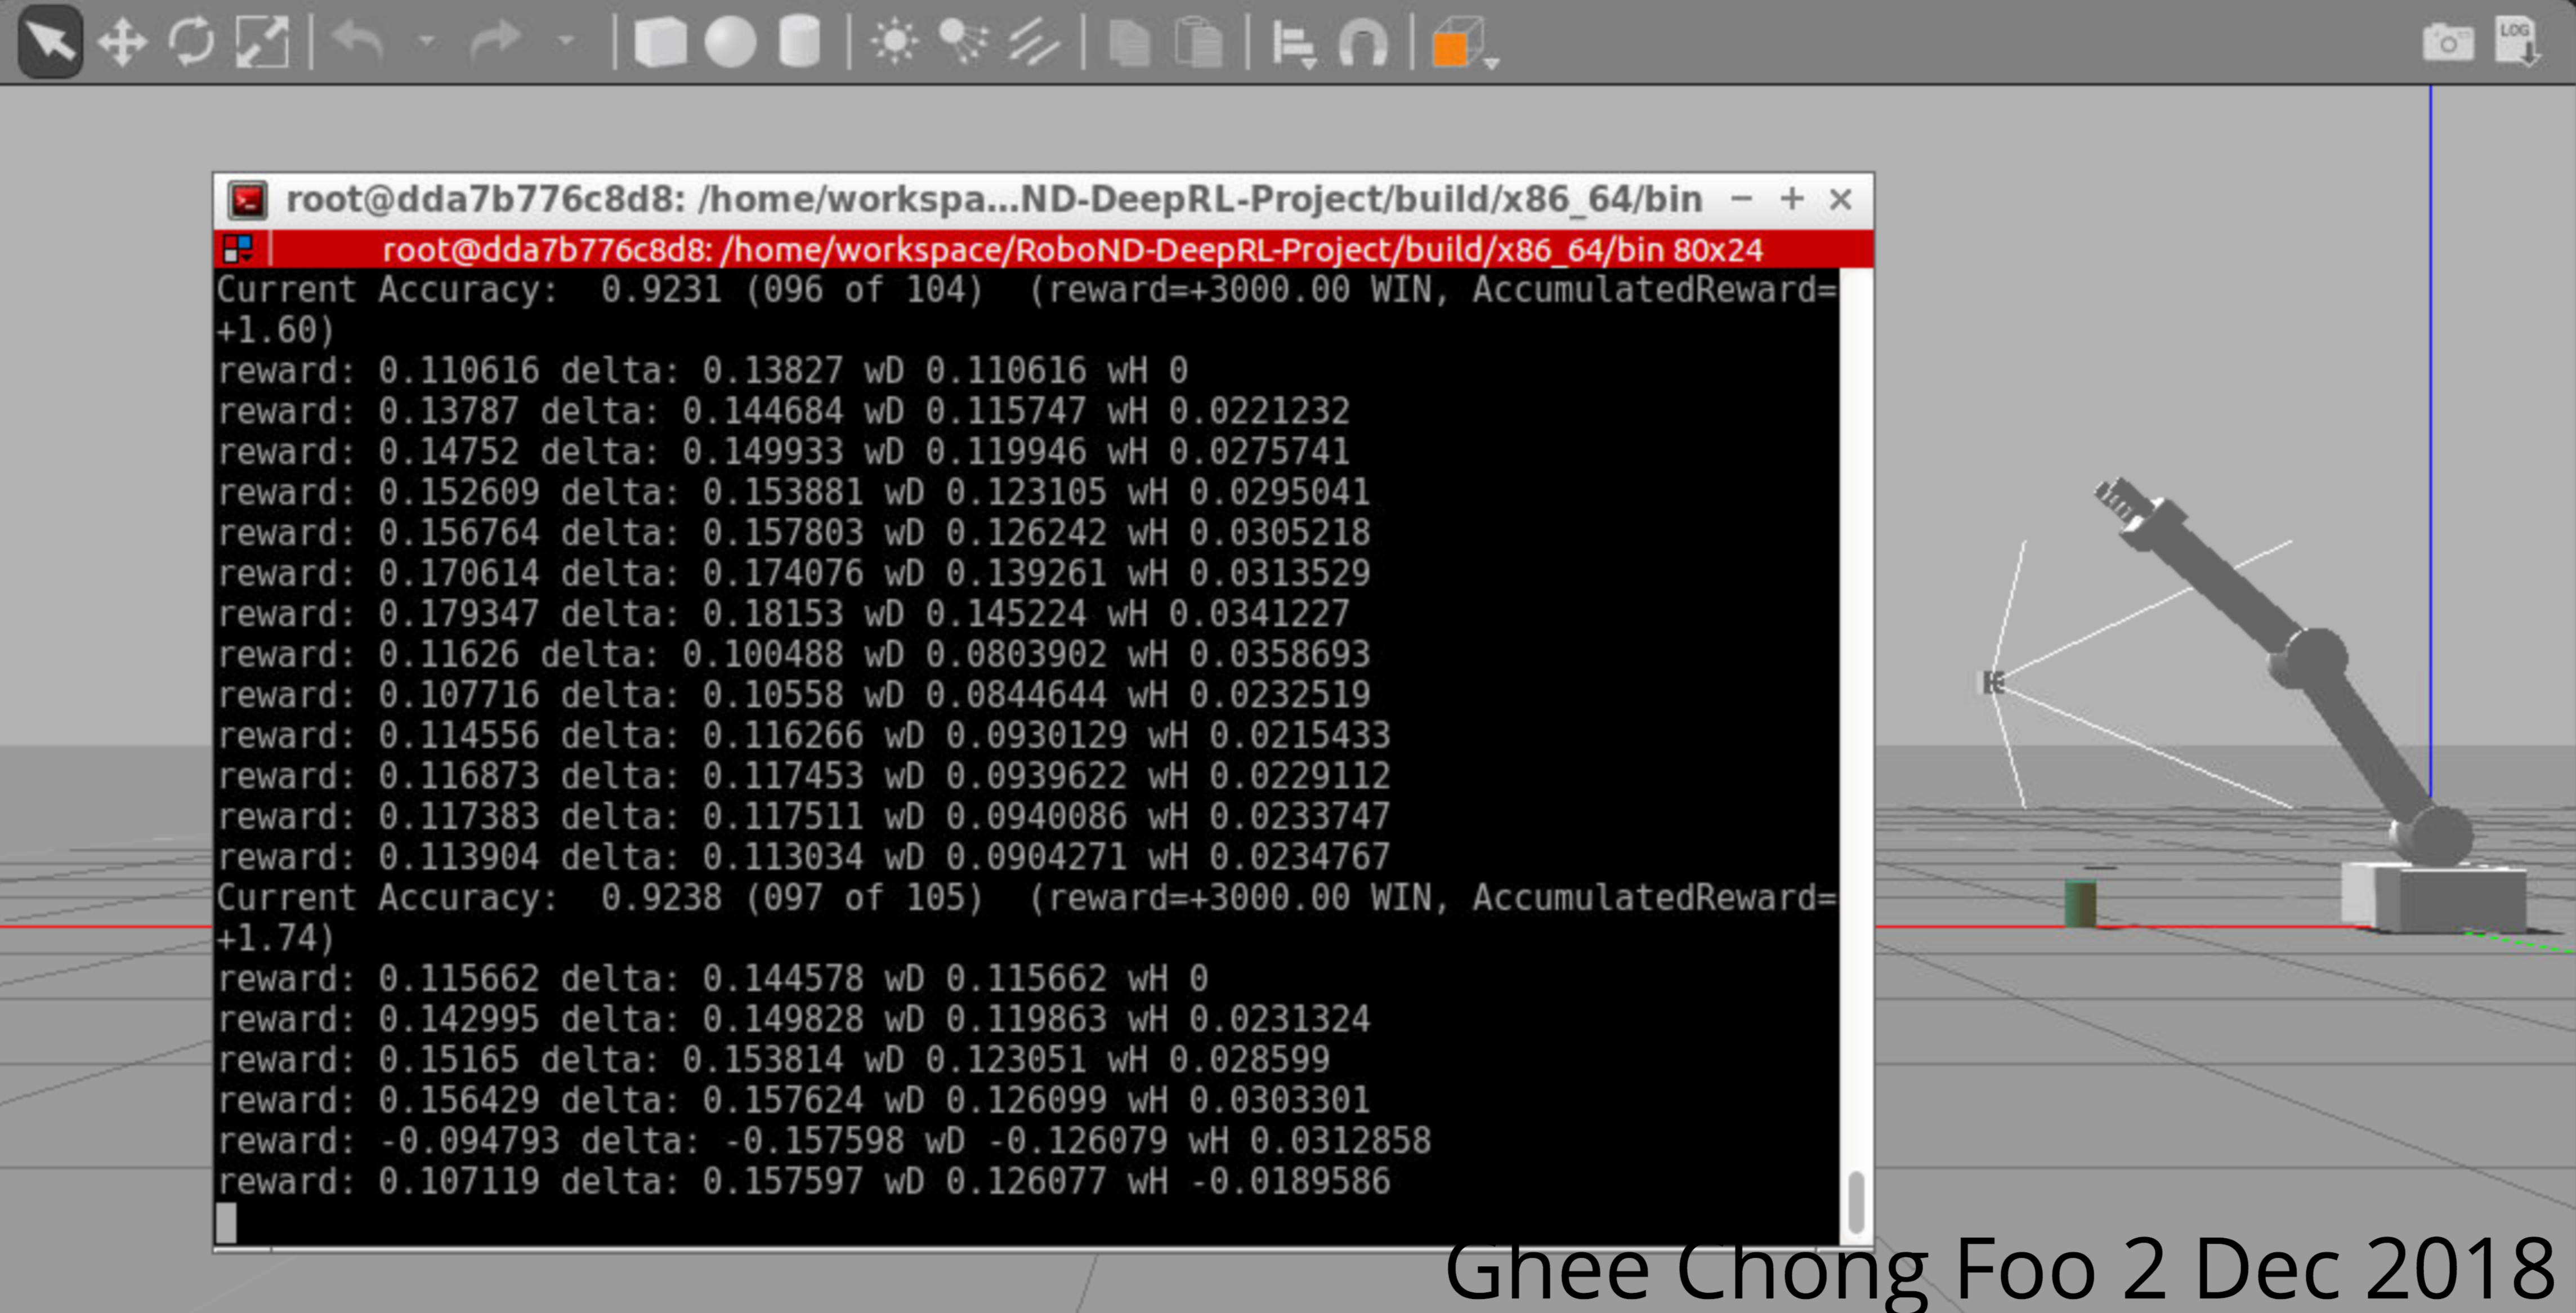
\includegraphics[width=\linewidth]{Challenge_1.png}
      \caption{Robotic Arm Touching Object with non-Gripper in Challenge 1}
      \label{fig:Challenge_1}
\end{figure}

\begin{figure}[thpb]
      \centering
      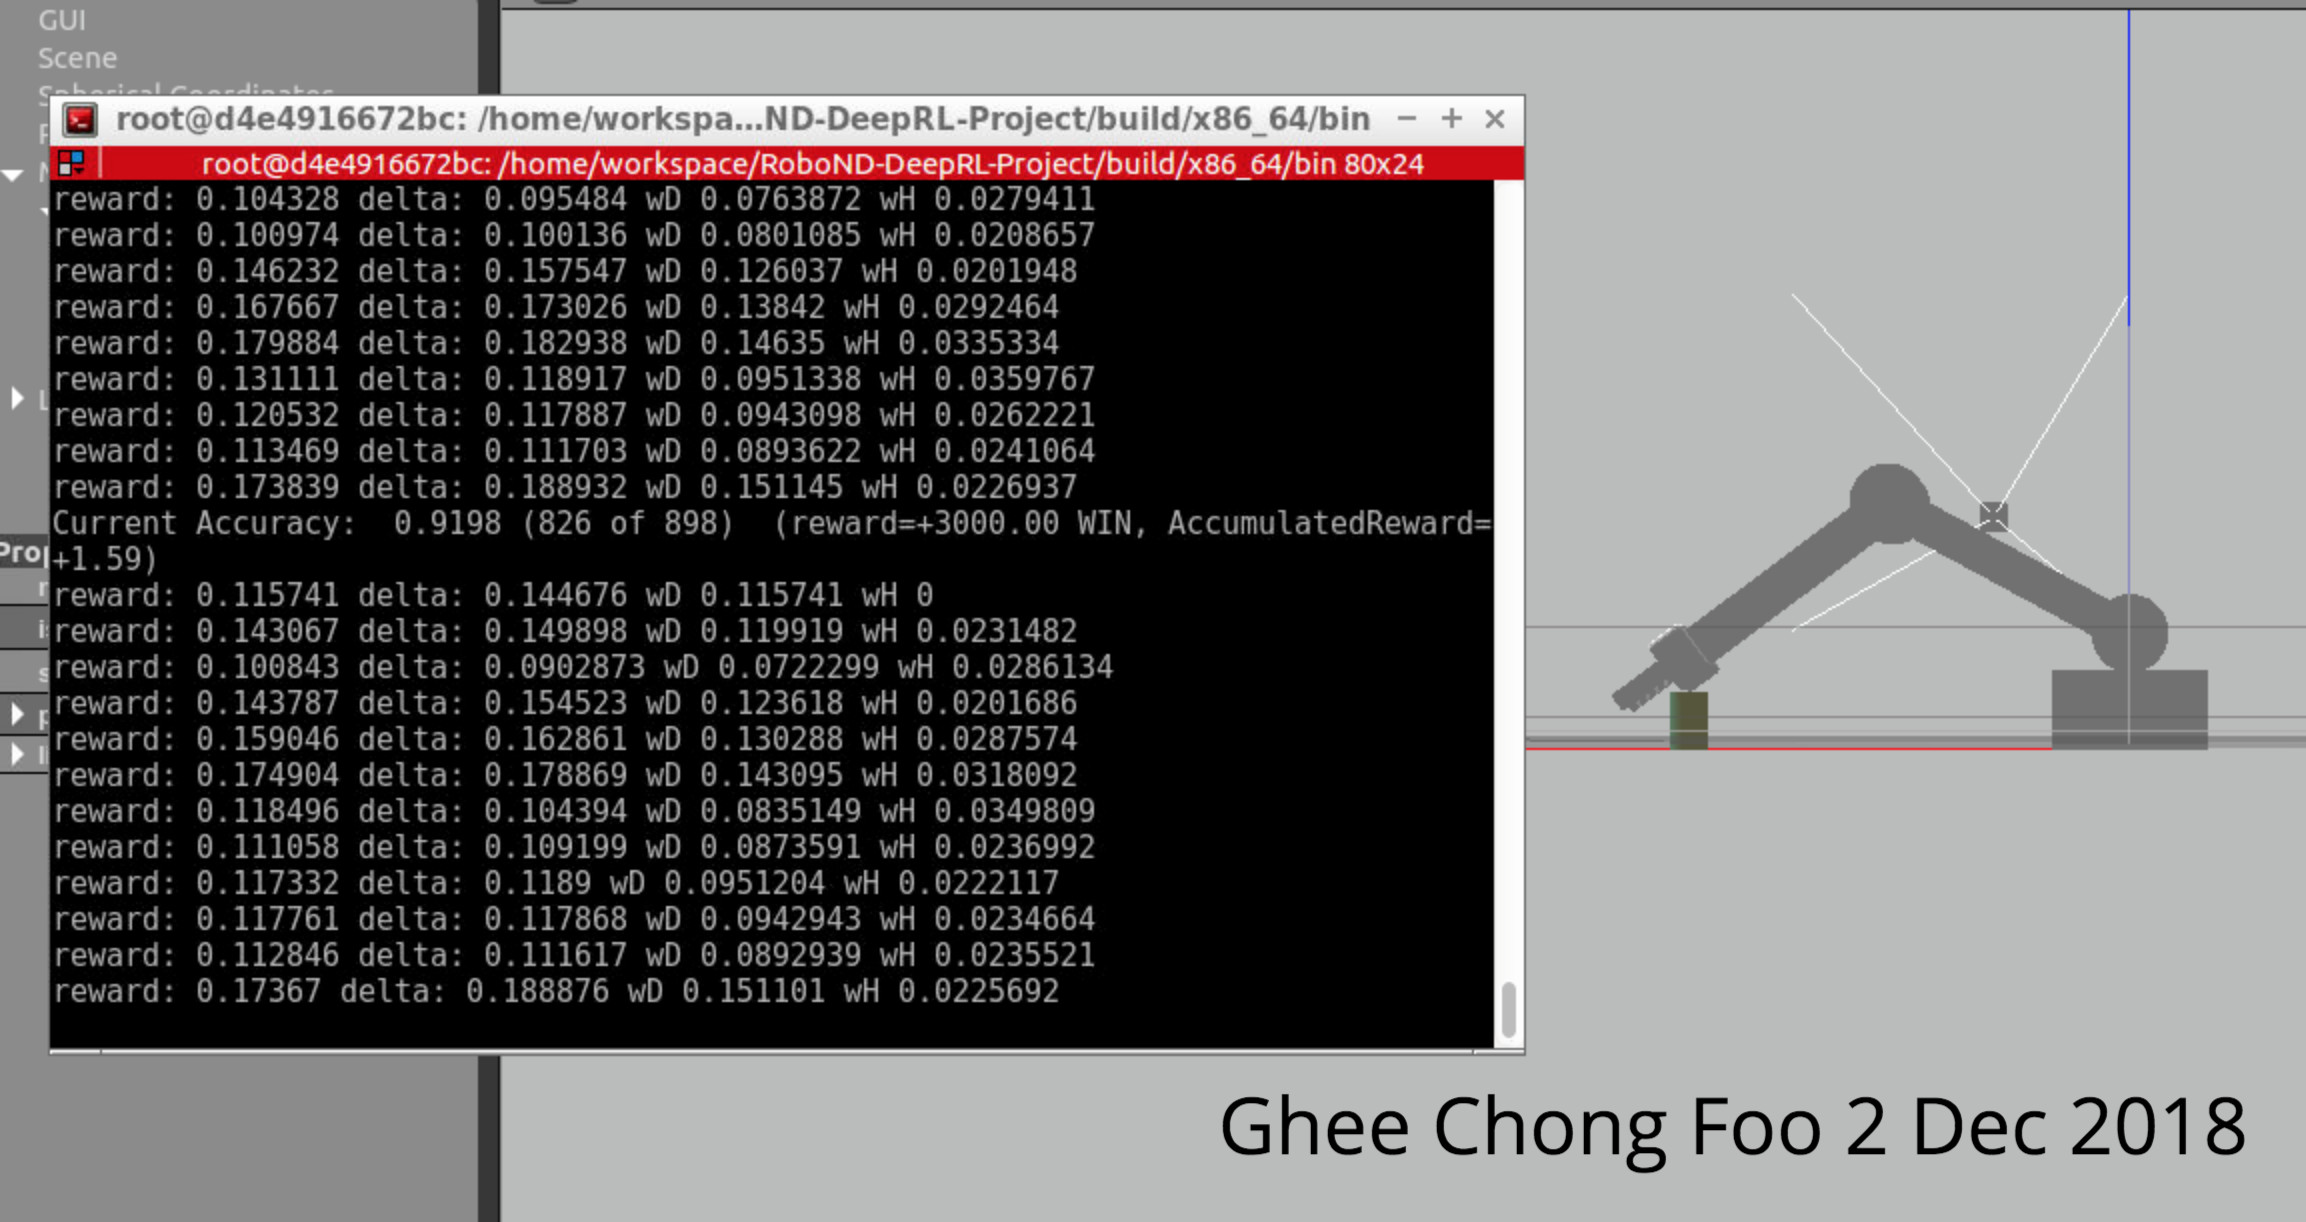
\includegraphics[width=\linewidth]{Challenge_2.png}
      \caption{Robotic Arm Touching Object with Gripper in Challenge 2}
      \label{fig:Challenge_2}
\end{figure}

%Results: Explain the results obtained for both objectives. Include discussion on the DQN agent's performance for both objectives. Include watermarked images, or videos of your results. Student should describe and briefly explain the results they achieved for both objectives. The discussion should also include their comments on the DQN agent's performance and if there were any shortcomings. Student should include either watermarked images of their results, or attach a video that displays the results and the arm in action.

\section{Discussion}
Training the DeepRL agent is a time consuming process which takes many hours of computing time. Same goes for hyperparameter tuning which might give different result for same setting, and one has to run the same setting multiple times to see the consistency, but might not few outlying results in particular run, i.e. one might observe a very poor accuracy in one run but a very high accuracy on another.  The consistency should converge should the agent was trained for longer hours, but this assumption is not able to be proved as often Udacity workspace timed out before longer hours of result can be observed.

\section{Future work}
%Future Work: Briefly discuss how you can improve your current results. Student should discuss on what approaches they could take to improve their results. 






\end{document}